\chapter{Design}\label{ch:design}

This chapter shall explain the design choices made while completing the project including the methods for calculating confidence, the format used to store transcription data, and the overall design of a demo system for computer-aided transcription.

\section{Speech Data}

According to its authors, Whisper's robustness is due likely in part to its use of a language model in its decoder\cite{whisper}.
Though likely beneficial for keeping track of sentence context, this poses a potential threat to the models accuracy in a number of circumstances, including;

\begin{itemize}
  \item Misspoken words or sentences with improper syntax (e.g. 'then' instead of 'than'), for these errors may be corrected by the model, despite being inaccurate to the original recording.
  \item Disjoint terms (e.g. 'book purple dish soap'), as such terms are highly unlikely to occur in sequence and thus the language model will not consider them a probable output.
\end{itemize}

To combat these drawbacks, this work will use a conversational speech corpus rather than one made of spoken disjoint terms.
While not representative of all speech, an argument can be made that the majority of speech which must be transcribed (e.g. conference recordings, courtroom hearings, lectures, etc.) has a maintained context throughout and is not significantly formed of disjoint terms, though the potential for disjoint terms to be present in a recording should be acknowledged as a potential area of weakness for Whisper.

\mycomment{
  Change this, sounds jank
  }
While introducing the corpus selected for this work that the original objective was to explore the impact of age-related changes to speech on ASR performance, and for this goal the \emph{LifeLUCID} corpus\cite{lifelucid} was determined to be the best match.
Despite the scope of the project having since changed, the data gathered fits the new objective very well, as it is formed of 52 recordings of conversations between 104 discrete speakers aged between 8 and 85 years old.
They are solving a 'spot-the-difference' task, and the data selected for this work was recorded in normal conditions (that is, they can hear and communicate with each other normally).

The corpus' authors mention that the reference transcripts were generated by an ASR system and only one channel's audio was human-corrected.
The ability to compare the quality of ASR output to a reference transcript is required to evaluate this work, thus, only the human-corrected transcript and corresponding audio channel were used to ensure the references are reliable.
This leaves 52 10-minute recordings of individual speakers with gaps where the other participant is speaking.

\subsection{TextGrid Format}

The reference transcripts are supplied in \emph{Praat TextGrid} format which is produced by the Praat software suite\cite{praat}.
The TextGrid format consists of each individual part of speech (words, hesitations, mid-sentence silences, silences when the other participant is speaking etc.) being present in consecutive entries with the time in the recording which they start and finish.

\begin{figure}[h!]
\centering
\begin{BVerbatim}
intervals [14]:
  xmin = 21.05 
  xmax = 21.47 
  text = "BUSH" 
\end{BVerbatim}
  \caption{Example of an entry in TextGrid format}
  \label{fig:textgrid-example}
\end{figure}

Figure \ref{fig:textgrid-example} is an example of a single 'interval' in the TextGrid format.
A larger example is available in Appendix \ref{appendix:textgrid}
You may observe that \texttt{xmin} and \texttt{xmax} denote the points in the recording at which the section starts and ends, and \texttt{text} denotes the content of the section.
Considering that each entry appears consecutively and that there are over 1,000 in each file, the format is not easily human-readable.

\subsection{Data Preparation}

There are a number of issues with using the data in its original format, including;

\begin{enumerate}
  \item Whisper struggles to maintain alignment when transcribing long form data\cite{whisper}, so the approximate 10-minute length of each recording requires shortening to maintain system performance;
  \item TextGrids are not human-readable; and
  \item The output of the ASR system should be stored alongside the reference transcripts to ease evaluation, which is not possible using TextGrids.
\end{enumerate}

The solution to the first problem would best be solved by splitting the conversation recordings into individual utterances.
Luckily, the human-evaluated references include metadata which shows the start- and stop-times of each word and non-word part of speech, meaning it can easily be split into individual utterances without using voice activation detection or other automatic techniques.
Using the documentation for LifeLUCID it was possible to determine that there are two types of non-speech token;

\begin{enumerate}
  \item 'Break' tokens -- these are tokens which denote the speaker is not mid-utterance; either listening to the other participant or engaged in irrelevant discussion (these latter parts are silenced in the recordings).
  \item 'Junk' tokens -- these denote either:
    \begin{itemize}
      \item The speaker has paused (but the other participant is not speaking).
      \item A bell or dog bark is being played as part of their task (these are silent in the recording).
      \item Hesitations (e.g., 'umm', 'uhhh', etc.)
      \item Other non-speech, non-breaking tokens (not specified in their documentation but present in the transcripts).
    \end{itemize}
\end{enumerate}

For the purpose of this work, an utterance is defined as an uninterrupted piece of speech without any long pauses.
By providing threshold values for the minimum length of a 'break' token and maximum length of a 'junk' token, the boundaries at which utterances start and end can be easily computed from the reference TextGrids.
The utterance boundaries can then be used to extract individual utterances from the full-length recordings, resulting in a series of numbered audio files.

The second and third problems can be solved together by changing from the TextGrid format to JSON (JavaScript Object Notation).
This format is human-readable\cite{nurseitov2009comparison} and able to hold all the data and metadata required for this work, including a way to reference the original piece of audio it represents.

\section{Running Whisper}

\mycomment{
  Would it be worth moving some of this to chap3? defining a 'target user' is probably better suited to there...
  }
Whisper comes packaged with models of various sizes, requiring between approximately 1 and 10GB of VRAM and an increasing amount of time to produce transcripts.
Considering the objective to create an automatic transcription system which uses entirely free and open-source software, it is worth assuming that the individuals or institutions who would benefit the most from this system are those without the resources to rely on professional manual transcription.
It follows, then, that these 'target users' would not have access to high-powered computers and instead rely on consumer-grade hardware to generate transcriptions.
Thus, for the purposes of this work, the medium English-language model was selected as it requires only 5GB of VRAM and takes approximately half as much time to produce transcripts as the larger models\cite{whisper}.

\section{Confidence Scoring}\label{sec:confidence-scoring}

Whisper does not have a clear confidence scoring system in its unaltered state.
This is a caveat for calculating confidence resulting from the design philosophy of Whisper's authors; it is a one-shot model so it is not expected to be fine-tuned to a dataset before use.
Without fine-tuning or prior exposure to the type of data present in the input, Whisper can't be trained to predict the correctness of its output.

Therefore, for it to be viably used to aid a human transcriber, some method to estimate system confidence must be implemented based on the way it converges on and scores an output.
At a high level, there are two sources from which to estimate confidence: Whisper's standard output, and its internal processes.

Table \ref{table:confidence-motivations} gives a brief comparison of the benefits and drawbacks associated with each of these sources of confidence;

\begin{table}[hb!]
\centering
\begin{tabular}{P{0.2\linewidth}  P{0.35\linewidth}  P{0.35\linewidth}}
\toprule
\textbf{Score Source} &
  \textbf{Benefits} &
  \textbf{Drawbacks} \\[0.3cm] \toprule
\textbf{Standard Model Output} &
  Does not require any modification to Whisper. &
  Only shows an average probability score per utterance. \\[0.7cm] \midrule
\textbf{Model Internal Scoring} &
  Allows access to per-word scoring and the steps the model takes to converge on an output. &
  Requires modification to Whisper. \\ \bottomrule
\end{tabular}
\caption{Comparison between sources of model confidence}
  \label{table:confidence-motivations}
\end{table}


The following subsections provide a detailed explanation of how each approach works and should help illustrate the benefits and drawbacks of each.

\subsection{Confidence From Model Output}

Though it does not yield a clear confidence score, Whisper does output various data relating to its processing of the input.
These include;

\begin{itemize}
  \item \texttt{avg\_logprob} -- The average of the $\log$ token-probability for a segment of speech (discussed further below)
  \item \texttt{compression\_ratio} -- The ratio of the length of the UTF-8-encoded text to its gzip-compressed representation.
    Due to the way gzip operates, this ratio indicates the 'repetetive-ness' of the decoded text; a higher ratio means that the result is more repetetive, suggesting that there may have been a decoding error.
  \item \texttt{temperature} -- Before producing an output, if the \texttt{avg\_logprob} is below a certain threshold or the \texttt{compression\_ratio} is above some threshold, the model will treat the decoding as failed and compute a new output with an increased temperature parameter.
    Temperature is used to introduce some randomness while computing predictions, therefore the higher the final output \texttt{temperature} value is, the more randomness had to be introduced in order to determine the given output.
  \item \texttt{no\_speech\_prob} -- Whisper is trained to complete many tasks, one of which being the detection of non-speaking moments in a recording.
    This value indicates the model's predicted probability that there is no speech in the input audio file.
\end{itemize}

Of these metrics, this work will focus on the \texttt{avg\_logprob}, which is the average of the $\log$ probabilities for each token in a segment of the input, which are computed as the $\log \softmax$ of the \emph{logits}, which can be thought of as unnormalised 'scores' that have been assigned to each token while decoding.
The $\softmax$ function is used to normalise these scores such that their sum is equal to $1$ (allowing them to be used as probabilities).

The logits themselves are calculated during each forward pass through the decoder, derived from both learned positional and token embeddings.
In the context of the Transformer's decoder, learned positional embeddings can be thought of as a way to learn information about token positions in the transcript\cite{wang2020position}.
By using token- and learned position-level weights with cross-attention from the encoder\cite{vaswani2017attention}, Whisper acts like an \say{audio-conditional language model}\cite{whisper}; the scores (logits) assigned to tokens are based on both the encoded audio input and a model of language.

\subsection{Confidence From Model Internals}

By default, the only information Whisper makes available about the probability scoring it used to decide on some output is \texttt{avg\_logprob} despite having internally computed scores for every token in the output.

The 'tokens' that have been refered to in this section are computed using the GPT-2 tokenizer from the \emph{tiktoken} library\cite{tiktoken}.
Words may be represented by one or more tokens called 'subword tokens' which are decoded by the tokenizer; the scores for each of these are different so a per-word score may be computed as the average score for each subword token in a word.

\begin{figure}[h]
  \centering
  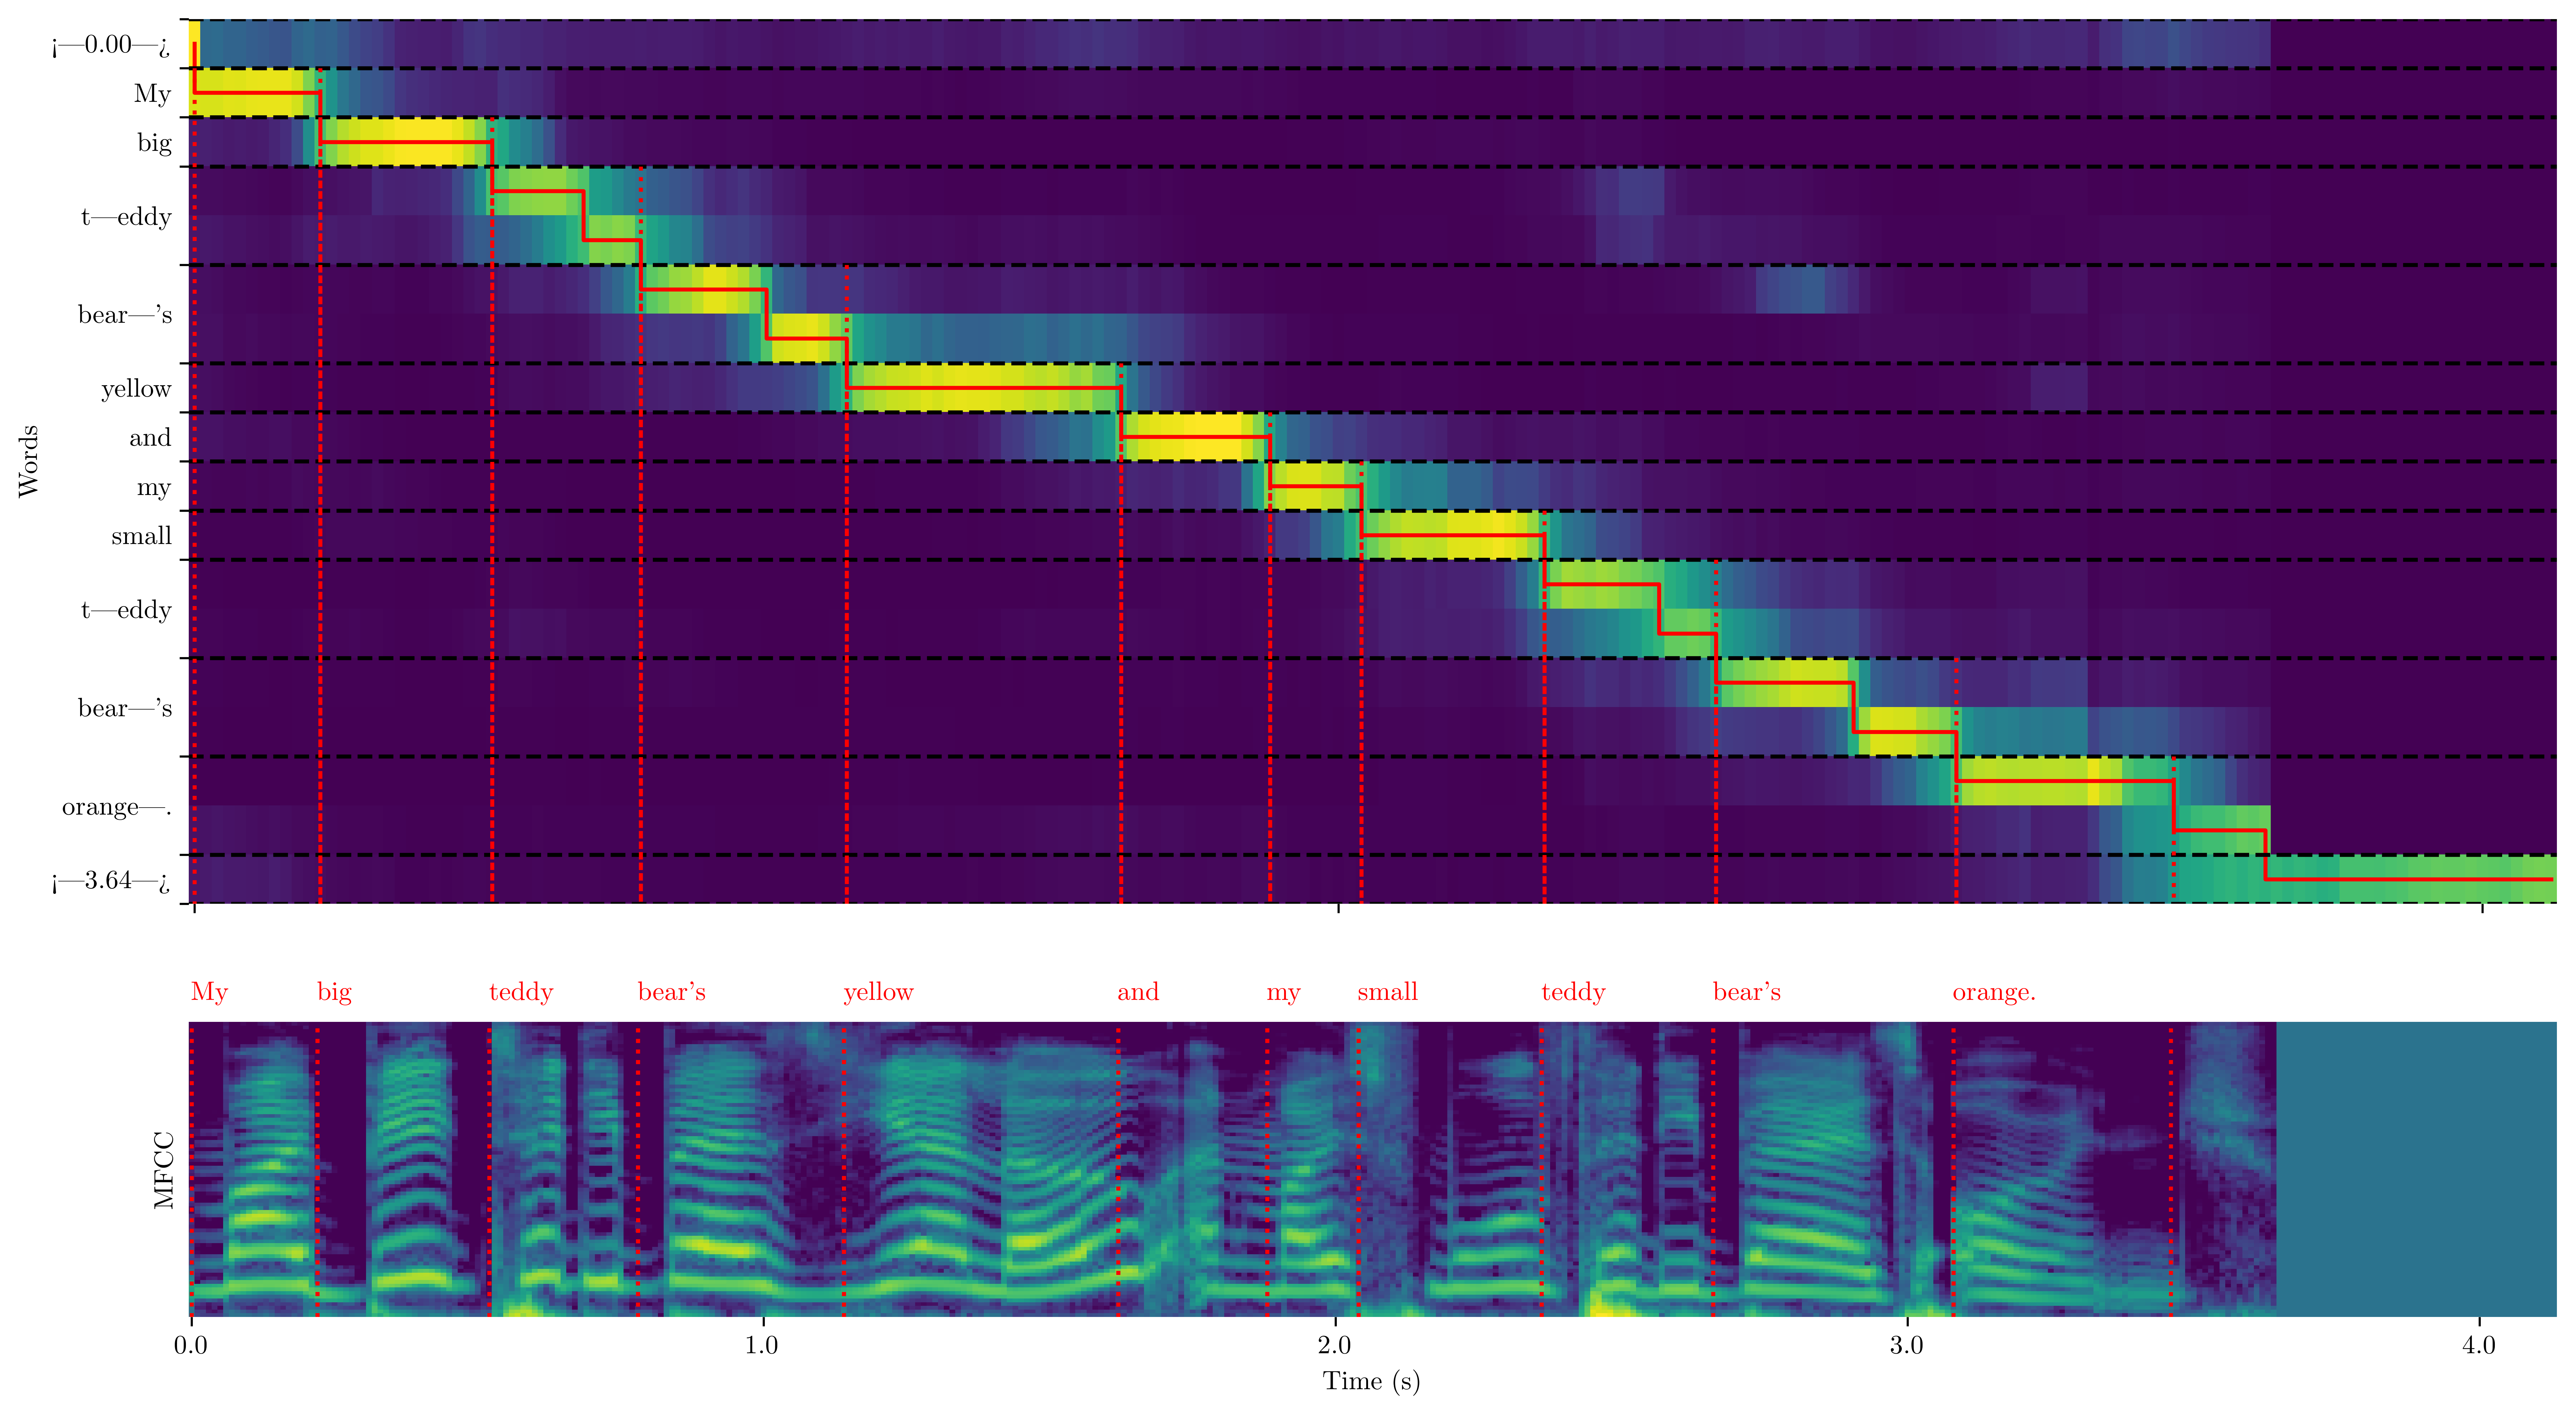
\includegraphics[width=\textwidth]{images/mfcc-with-words.png}
  \caption{Word alignments example}
  \label{fig:word-alignments-example}
\end{figure}

Figure \ref{fig:word-alignments-example} was generated using the \emph{whisper-timestamped} library\cite{whisper-timestamped, whisper-ts-dtw-paper, whisper}.
The top plot shows \say{the transformation of cross-attention weights used for the [word] alignment}\cite{whisper-timestamped}.
Notice that the words 'teddy' and 'bears' are split into subwords.

The aforementioned \emph{whisper-timestamped} library is able to assign confidence scores to each word, computed as the exponential of the mean of the $\log$ probabilities of each subword token in a given word.
Though based on probability scores which may not be wholly representative of confidence (as discussed in section \ref{sec:litreview-confidence}), operating on individual words rather than whole utterances should provide more detail of the per-word scores than \texttt{avg\_logprob} does.

\section{A System For Transcription}

As discussed in the requirements chapter (section \ref{sec:req-design-system}), this work would benefit greatly from a piece of software which serves to demonstrate computer-aided transcription.
At a basic level, the software should enable a user to sort utterances in a conversation by some estimation of confidence to allow them to manually correct the ASR-generated transcripts in non-descending order of correctness.

\begin{figure}[h]
  \centering
  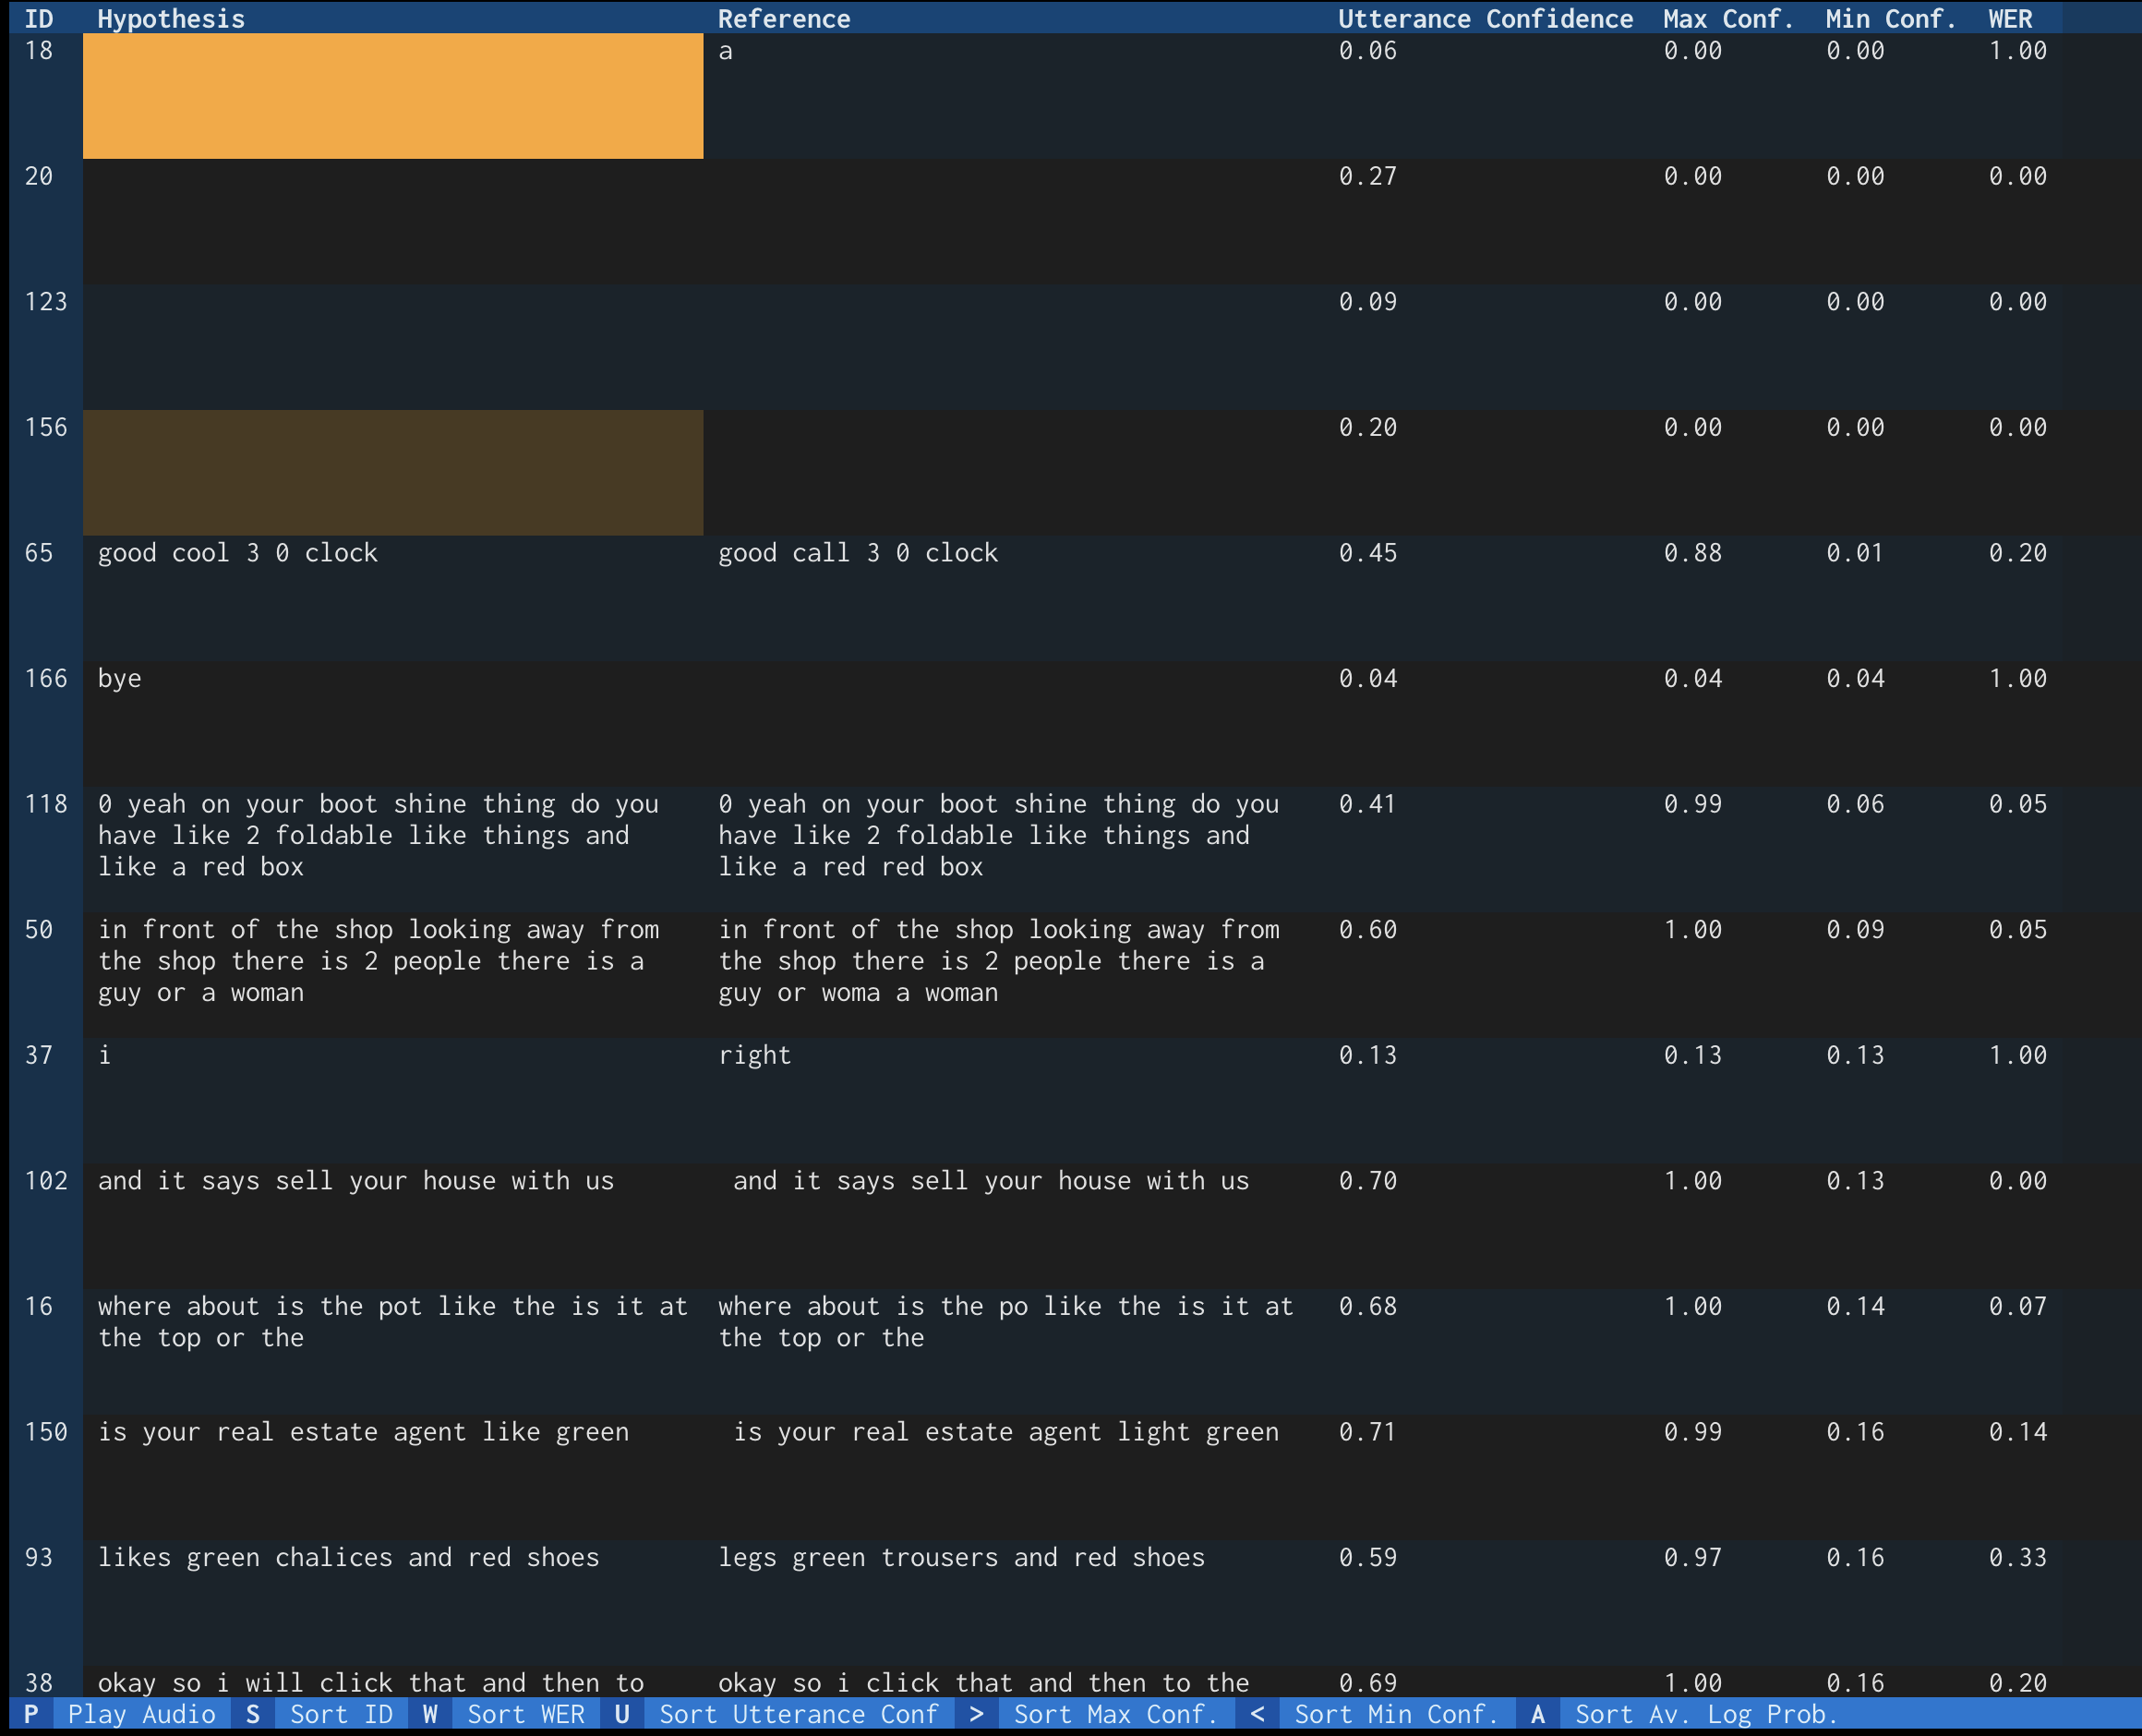
\includegraphics[width=\textwidth]{images/confidence-order.png}
  \caption{Utterances in confidence order.}
  \label{fig:sys-confidence}
\end{figure}

If there is any question about the context of a section of speech (e.g. there are unclear or  parts of speech), the user may return to chronological order and assess the surrounding utterances for information.

\begin{figure}[h]
  \centering
  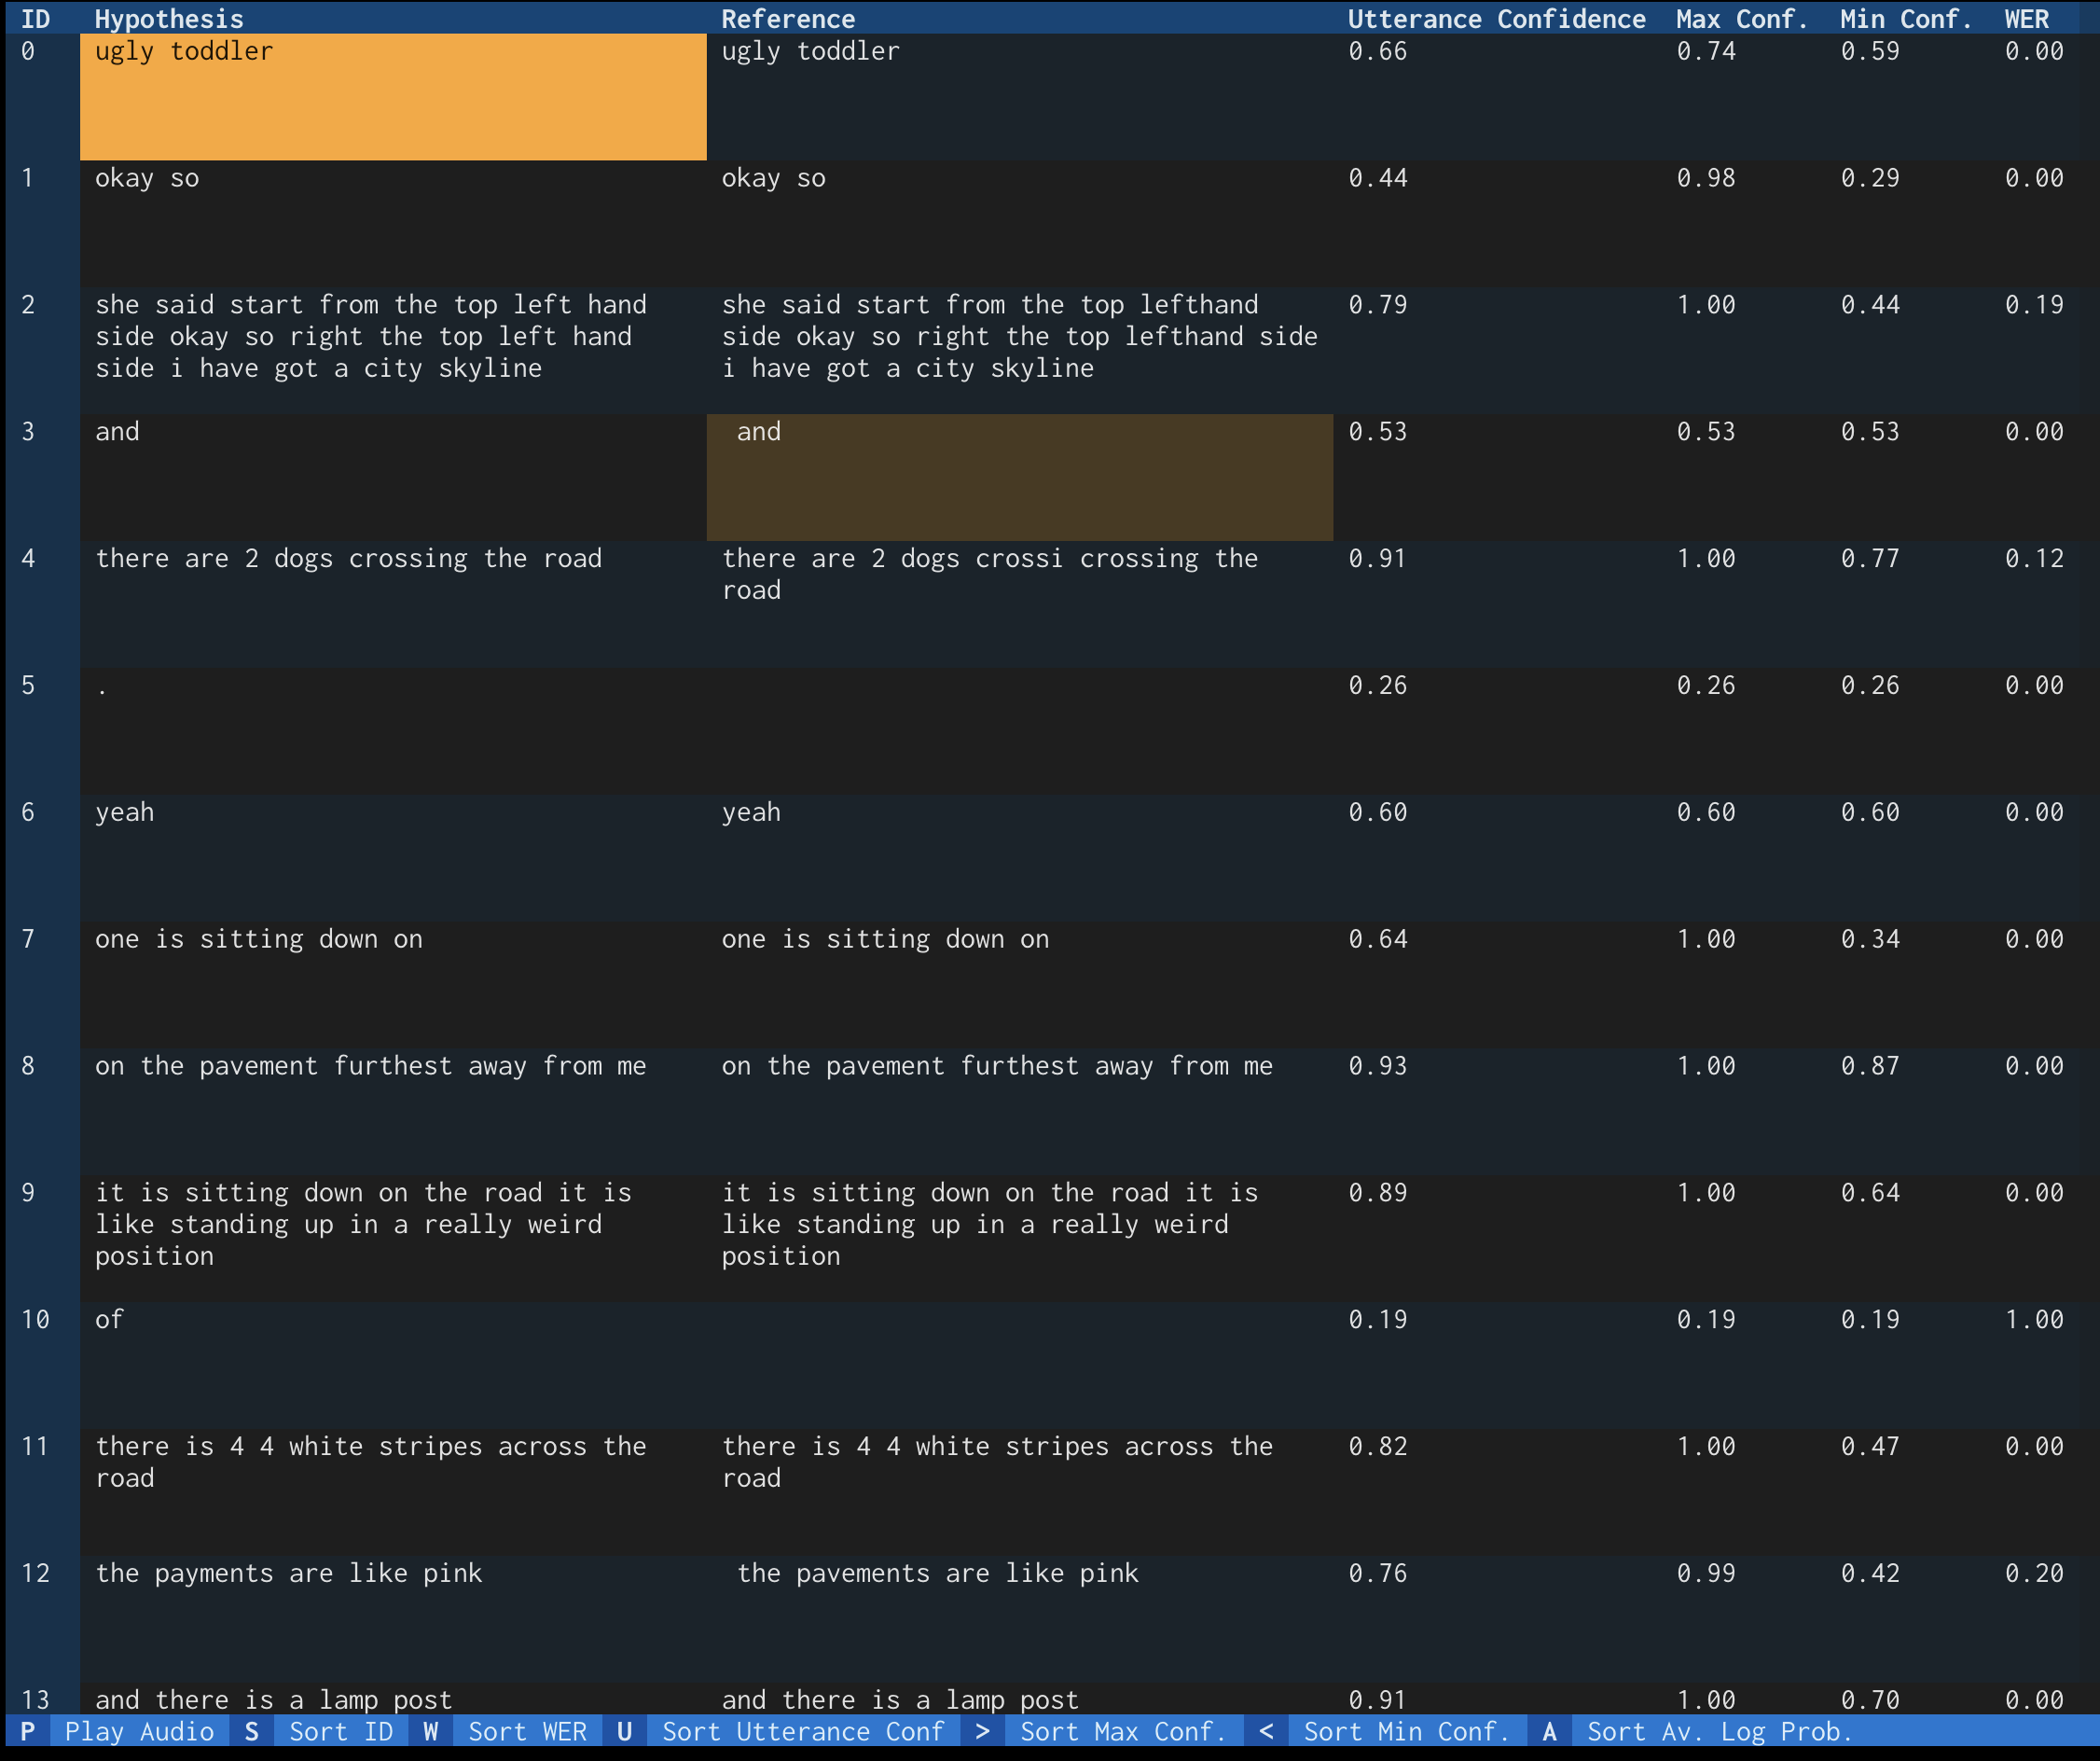
\includegraphics[width=\textwidth]{images/chronological-order.png}
  \caption{Utterances in chronological order.}
  \label{fig:sys-chronological}
\end{figure}

A user may be influenced by the ASR transcript if they read it while listening to the accompanying audio.
To solve this, words may be 'blanked out' depending on their assigned confidence score, those below a threshold parameter are replaced by blank sections so the user can't be conditioned by what the ASR predicted the output to be.

\begin{figure}[h]
  \centering
  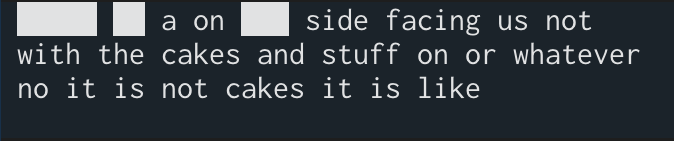
\includegraphics[width=\textwidth]{images/text-blanking.png}
  \caption{Example of a 'blanked out' utterance.}
  \label{fig:sys-blanking}
\end{figure}

Displaying word-level confidence scores for every word in a sentence is not an intuitive way to interact with a computer system; instead, by colouring the words based on their assigned confidence score, the user may provide corrections to words which are considered less likely to be correct than others.

\begin{figure}[h]
  \centering
  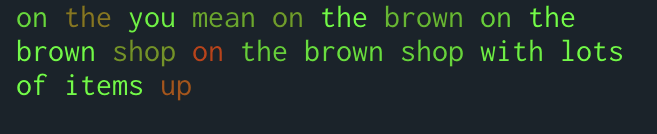
\includegraphics[width=\textwidth]{images/text-highlighting.png}
  \caption{Example of an utterance with confidence-based highlighting.}
  \label{fig:sys-highlighting}
\end{figure}

All of these options may be selected using a simple menu.

\begin{figure}[h]
  \centering
  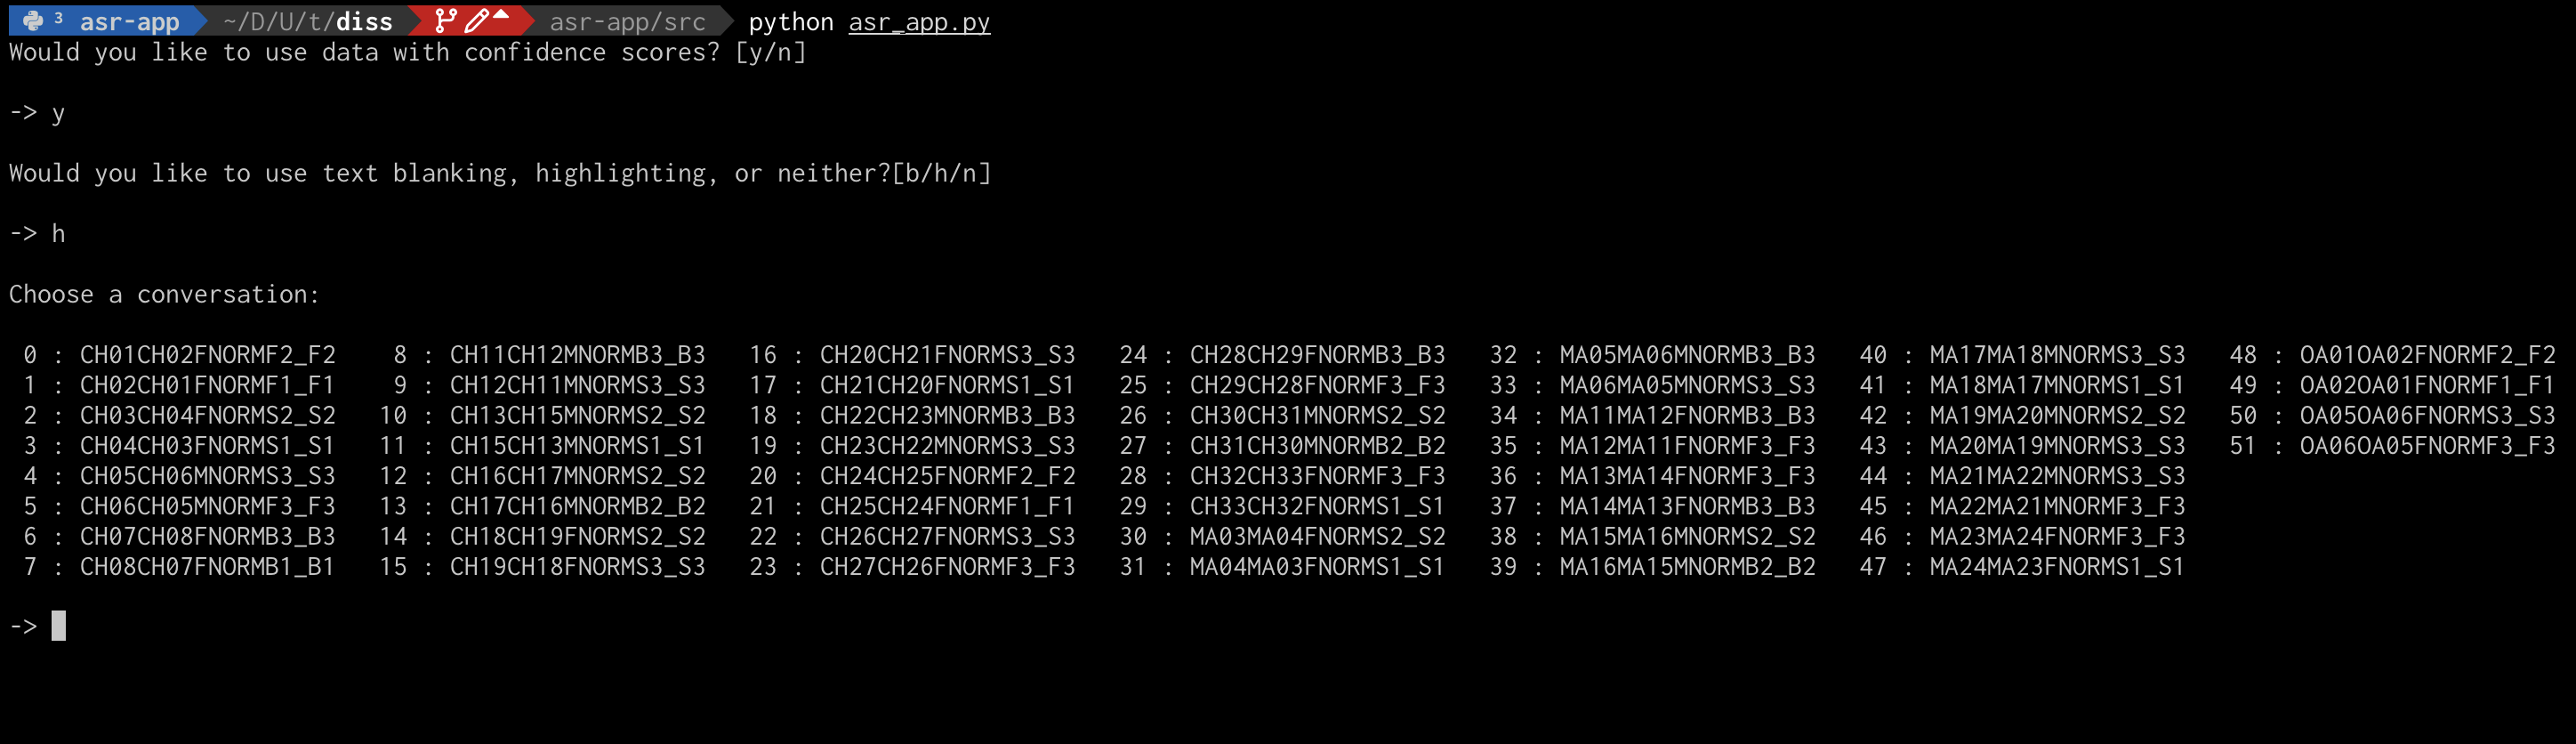
\includegraphics[width=\textwidth]{images/menu.png}
  \caption{Menu presented to a user before starting the application.}
  \label{fig:sys-menu}
\end{figure}

This system is not capable of taking input from a user, rather it exists with the purpose of providing an example to build a more fully-featured computer-aided transcription from.
It is run in a terminal window using Python with the following packages;

\begin{itemize}
  \item \emph{Textual}\cite{textual} to build the application front-end,
  \item \emph{pysoundfile}\cite{pysoundfile} and \emph{python-sounddevice}\cite{pysounddevice} to load and play audio clips, and
  \item \emph{Rich}\cite{rich} to enable text highlighting in the terminal.
\end{itemize}
